% Provenance (never printed): see sources/outline_sources.md (Year 3:
% radial velocity, transits, imaging and microlensing; what has been
% found; atmospheres from transmission spectra).
% Brief: sources/book5/BRIEFS.md, ch. 28. Curves from figdata/bachelor-3/
% rv_transit.py (Keplerian radial-velocity curves, a limb-darkened transit
% light curve computed by numerical integration, point-lens microlensing)
% and exoplanet_archive.py (the NASA Exoplanet Archive's composite table of
% confirmed planets, fetched 2026-10-23, with the model mass--radius curves
% of Zeng et al.). Exercise and problem values in the Book 5 scratch
% calculator calc/ch28.py. Selene's Lamp and its planet are invented.
\chapter{Eksoplanet}\label{ch:b3:exoplanets}

Pada musim gugur 1994, dua astronom yang mengukur kecepatan 142
bintang menemukan bahwa salah satunya, 51~Pegasi, bergerak mendekat dan menjauh
dari kita dengan periode sekitar empat hari. Semi-amplitudo gerak itu
\qty{59}{m.s^{-1}}, empat kali lipat dari yang dapat dideteksi spektrograf mereka. Benda
yang menarik bintang itu bermassa paling sedikit setengah massa
Jupiter, pada orbit \qty{0.05}{au}, delapan kali lebih dekat ke bintangnya
daripada Merkurius ke Matahari. Tidak ada teori formasi planet yang memberi tempat bagi
benda seperti itu. Penemuan yang diumumkan pada Oktober 1995 ini membuka bidang baru
astronomi: tiga dekade kemudian, lebih dari enam ribu planet di sekitar
bintang lain telah dikonfirmasi, beberapa di antaranya telah teramati langsung, dan
atmosfer sebagian di antaranya telah dianalisis. Bab ini menunjukkan bagaimana planet
yang terlalu redup untuk dilihat ditemukan, apa yang telah ditemukan, dan bagaimana atmosfernya
dibaca.
% ledger: nobel19:51peg, planet:Mercury.dist, data:b5-pscomp

\begin{recall}
Efek Doppler, kecepatan radial, bintang biner spektroskopik, hukum Kepler,
masalah dua benda dan pusat massanya, hukum Planck, dan
tinggi skala atmosfer isotermal ada di buku fisika. Eksoplanet
dan zona layak huni bintang ada di buku sekolah. Fluks
dan luminositas suatu sumber ada di volume Tahun 1, dalam
bab tentang teleskop dan fotometri; suhu kesetimbangan, dalam
bab tentang planetologi komparatif. Formasi planet dan garis salju
ada di volume Tahun 2. Jeans dan \omterm{def:b3:planetary-atmospheres:hydrodynamic}{lolos hidrodinamik} serta batas
zona layak huni ada di volume ini, pada bab tentang
atmosfer planet.
\end{recall}

\section{Metode kecepatan radial}\label{sec:b3:exoplanets:rv}

Planet tidak mengorbit bintangnya semata: keduanya mengelilingi pusat massa bersama.
Bintang, yang jauh lebih berat, bergerak pada orbit kecil sendiri, dan cahayanya
mengalami pergeseran Doppler bolak-balik dengan periode planet.

\begin{definition}[Metode kecepatan radial; massa minimum]\label{def:b3:exoplanets:rv}
Yang disebut \emph{metode kecepatan radial}\index{metode kecepatan radial} mendeteksi
planet dari variasi periodik kecepatan radial bintangnya,
yang diukur dari pergeseran Doppler garis-garis spektrum bintang. Jika
inklinasi $i$ orbit terhadap bidang langit tidak diketahui, maka
metode ini hanya mengukur $m_p\sin i$, hasil kali massa planet dengan sinus
inklinasinya, yaitu \emph{massa minimum}\index{massa minimum}
planet.
\end{definition}

\begin{theorem}[Semi-amplitudo kecepatan radial]\label{thm:b3:exoplanets:semi-amplitude}
Bintang bermassa $M_\star$ dan planet bermassa $m_p$ pada orbit lingkaran
periode $P$, dengan inklinasi $i$, memberikan bintang kecepatan radial
$v_r(t) = \gamma + K\cos\bigl(2\pi(t - t_0)/P\bigr)$, dengan $\gamma$ adalah
kecepatan pusat massa, dan semi-amplitudo
\[
K = \left(\frac{2\pi G}{P}\right)^{1/3}
    \frac{m_p\sin i}{(M_\star + m_p)^{2/3}} .
\]
Pada orbit dengan eksentrisitas $e$, kurva tidak lagi berbentuk sinusoid,
$v_r = \gamma + K\bigl[\cos(\nu + \omega) + e\cos\omega\bigr]$, dengan $\nu$
anomali sejati dan $\omega$ argumen periastron, dan $K$
dibagi dengan $\sqrt{1 - e^2}$.
\end{theorem}

\begin{proof}
Untuk orbit lingkaran: jarak $a$ antara kedua benda mematuhi
hukum Kepler ketiga, $a^3 = G(M_\star + m_p)P^2/4\pi^2$. Bintang berada
pada jarak $a_\star = a\,m_p/(M_\star + m_p)$ dari pusat massa
dan menempuh lingkarannya dengan laju $v_\star = 2\pi a_\star/P$. Oleh karena itu
\[
v_\star = \frac{2\pi}{P}\,\frac{m_p}{M_\star + m_p}
          \left(\frac{G(M_\star + m_p)P^2}{4\pi^2}\right)^{1/3}
        = \left(\frac{2\pi G}{P}\right)^{1/3}\frac{m_p}{(M_\star + m_p)^{2/3}} .
\]
\omterm{def:b3:remote-sensing-gis:insar}{Garis pandang} membentuk sudut $\pi/2 - i$ terhadap bidang
orbit, sehingga hanya $v_\star\sin i$ dari kecepatan bintang yang sejajar dengannya, dan
komponen itu berputar bersama bintang: $v_r - \gamma = v_\star\sin i\,
\cos\bigl(2\pi(t - t_0)/P\bigr)$. Bentuk untuk orbit eksentrik diturunkan dari
elips Kepler dan diterima tanpa pembuktian.
\end{proof}

Karena planet jauh lebih ringan daripada bintangnya, $K$ menentukan $m_p\sin i$
begitu periodenya diukur dan massa bintang diketahui dari
spektrumnya. Untuk 51~Pegasi~b, $K = \qty{59}{m.s^{-1}}$ dan $P = \qty{4.23}{d}$
mengitari bintang bermassa satu massa Matahari memberi $m_p\sin i = 0.47$ massa Jupiter.
Jupiter menggerakkan Matahari sebesar \qty{12.5}{m.s^{-1}} selama
orbitnya yang \num{4331}~hari: pengamat jauh akan melihat kecepatan Matahari berayun sekitar
\qty{\pm 13}{m.s^{-1}} selama dua belas tahun. Bumi menggerakkan Matahari sebesar
\qty{9}{cm.s^{-1}}. Spektrograf yang menemukan 51~Pegasi~b mencapai
\qty{13}{m.s^{-1}}; penerusnya mencapai sekitar \qty{1}{m.s^{-1}} (setara
kecepatan jalan kaki \qty{3.5}{km/h}), dan yang terbaru dirancang untuk sekitar
\qty{10}{cm.s^{-1}}, cukup untuk planet bermassa Bumi di zona layak huni
bintang bermassa rendah, tempat orbit planetnya pendek dan bintangnya pun bermassa rendah.
Bintang itu sendiri menetapkan batas bawah: denyut dan bintik permukaannya,
yang terbawa berputar oleh rotasinya, juga menggeser garis-garis spektrumnya, dan sinyal planet
harus dibedakan darinya.
% ledger: nobel19:51peg, nobel19:sun-jupiter, nobel19:migration, planet:Jupiter.mass, planet:Jupiter.Porb, planet:Jupiter.ecc, planet:Earth.mass, sun:mass, eso:espresso, const:G

\begin{omfigure}
\centering
\begin{tikzpicture}
\begin{axis}[width=0.86\linewidth, height=0.40\linewidth,
  xmin=0, xmax=2, ymin=-40, ymax=42,
  xlabel={fase orbit (dalam periode)}, ylabel={$v_r - \gamma$ (\unit{m.s^{-1}})},
  tick label style={font=\scriptsize}, label style={font=\small},
  legend style={font=\scriptsize, at={(0.5,-0.30)}, anchor=north, legend columns=2, draw=none, cells={anchor=west}, /tikz/every even column/.append style={column sep=1em}}]
\addplot[thin, black!40, forget plot] coordinates {(0,0) (2,0)};
\addplot[thick, omDef] table[x=phase, y=v_circ] {figdata/out/bachelor-3-rv_transit-rv.dat};
\addlegendentry{orbit lingkaran}
\addplot[thick, dashed, red!70!black] table[x=phase, y=v_ecc] {figdata/out/bachelor-3-rv_transit-rv.dat};
\addlegendentry{$e = 0.3$, $\omega = \ang{60}$}
\draw[<->, thick] (axis cs:1.0,0) -- (axis cs:1.0,30);
\node[font=\scriptsize, anchor=east] at (axis cs:0.99,12) {$K$};
\end{axis}
\end{tikzpicture}
\par\smallskip{\small Kecepatan radial suatu bintang dengan satu planet, selama
dua orbit, untuk planet rekaan dengan $K = \qty{30}{m.s^{-1}}$ dan
periode sepuluh hari. Pada orbit lingkaran (garis utuh), kurvanya berbentuk sinusoid
dengan semi-amplitudo $K$. Pada orbit eksentrik (putus-putus) bintang bergerak
paling cepat di dekat periastron, dan kurva menjadi tak simetris: ekstremnya adalah
$K(1 \pm e\cos\omega)$ dan ayunan puncak-ke-puncak tetap
$2K$.}\label{fig:b3:exoplanets:rv}
\end{omfigure}

\section{Transit}\label{sec:b3:exoplanets:transits}

Jika orbit terlihat hampir sejajar dengan garis pandang, planet melintas di depan
bintangnya sekali setiap orbit dan menutupi sebagian kecil piringannya.

\begin{definition}[Metode transit; kedalaman transit; parameter tumbukan]\label{def:b3:exoplanets:transit}
Yang disebut \emph{metode transit}\index{metode transit} mendeteksi planet melalui
peredupan berkala cahaya bintangnya ketika planet melintasi piringan bintang. Adapun
\emph{kedalaman transit}\index{kedalaman transit} $\delta$ adalah
penurunan fraksional fluks bintang selama transit. Yang disebut \emph{parameter
tumbukan}\index{parameter tumbukan (transit)} $b = a\cos i/R_\star$ adalah
jarak terkecil antara pusat planet dan pusat bintang, sebagaimana terlihat
di langit, dalam satuan jari-jari bintang $R_\star$, untuk orbit dengan
jari-jari $a$ dan inklinasi $i$.
\end{definition}

\begin{proposition}[Kedalaman transit]\label{prop:b3:exoplanets:depth}
Sebuah planet gelap berjari-jari $R_p$ yang sepenuhnya di depan bintang dengan
kecerahan seragam memberikan kedalaman $\delta = (R_p/R_\star)^2$.
\end{proposition}

\begin{proof}
Planet menutupi luas $\pi R_p^2$ dari piringan yang luasnya $\pi R_\star^2$
yang kecerahannya sama di mana-mana; fluksnya turun sebanding.
\end{proof}

Jupiter yang melintasi Matahari akan meredupkannya \qty{1.06}{\percent}, Bumi
sebesar \num{84} bagian per juta: yang pertama dapat dijangkau teleskop kecil,
yang kedua memerlukan teleskop antariksa yang mengukur ribuan
bintang selama bertahun-tahun. Namun, piringan bintang tidak seragam.

\begin{definition}[Penggelapan tepi]\label{def:b3:exoplanets:limb}
Yang disebut \emph{penggelapan tepi}\index{penggelapan tepi} adalah penurunan kecerahan permukaan
bintang dari pusat piringannya ke tepinya.
Di dekat tepi, garis pandang memasuki atmosfer bintang secara miring
dan mencapai kedalaman optik satu di lapisan yang lebih tinggi dan lebih dingin, yang memancarkan
lebih sedikit. Ini sering ditulis sebagai hukum kuadratik dalam $\mu = \cos\theta =
\sqrt{1 - r^2}$, dengan $r$ jarak dari pusat piringan dalam
satuan jari-jari bintang: $I(\mu)/I(1) = 1 - u_1(1 - \mu) - u_2(1 - \mu)^2$.
\end{definition}

Planet yang dekat pusat piringan dengan \omterm{def:b3:exoplanets:limb}{penggelapan tepi} menutupi cahaya yang lebih terang
daripada rata-rata dan memperdalam transit; di dekat tepi, planet menutupi lebih sedikit. Dasar
kurva cahaya membulat dan tepinya melunak. Durasi
transit membawa informasi tentang geometri.

\begin{theorem}[Durasi transit]\label{thm:b3:exoplanets:duration}
Untuk orbit lingkaran dengan periode $P$, jari-jari $a$, dan inklinasi $i$, dengan
$p = R_p/R_\star$ dan \omterm{def:b3:exoplanets:transit}{parameter tumbukan} $b$, waktu dari kontak pertama
hingga kontak terakhir adalah
\[
T_{14} = \frac{P}{\pi}\arcsin\!\left(\frac{R_\star}{a}\,
          \frac{\sqrt{(1 + p)^2 - b^2}}{\sin i}\right),
\]
dan waktu antara kontak kedua dan ketiga, ketika planet berada
sepenuhnya di dalam piringan, $T_{23}$, diberikan oleh rumus yang sama dengan
$1 - p$ menggantikan $1 + p$.
\end{theorem}

\begin{proof}
Misalkan $\varphi = 2\pi t/P$ adalah fase orbit yang dihitung dari tengah transit.
Diproyeksikan pada langit, dengan $x$ sepanjang lintasan planet dan $y$ melintang terhadapnya,
pusat planet berada pada $x = a\sin\varphi$ dan $y = a\cos i\cos\varphi$
dari pusat bintang. Dalam satuan jari-jari bintang, kuadrat jarak adalah
\[
z^2 = \left(\frac{a}{R_\star}\right)^2(\sin^2\varphi + \cos^2 i\cos^2\varphi)
    = \left(\frac{a}{R_\star}\right)^2\sin^2 i\,\sin^2\varphi + b^2 .
\]
Kedua piringan bersentuhan dari luar saat $z = 1 + p$, yaitu pada
$\sin\varphi = \sqrt{(1 + p)^2 - b^2}\,R_\star/(a\sin i)$, simetris
terhadap tengah transit. Transit berlangsung selama fase $2\varphi$, yaitu
waktu $2\varphi P/2\pi = P\varphi/\pi$. Dengan $z = 1 - p$, kedua piringan bersentuhan
dari dalam.
\end{proof}

Untuk orbit lebar, arkus sinus sama dengan argumennya: $T_{14} \approx (P/\pi)
(R_\star/a)\sqrt{(1 + p)^2 - b^2}$. Transit di tengah berlangsung paling lama; yang
menyerempet, dengan $b$ dekat $1 + p$, singkat dan berbentuk V. Dengan mengukur
$T_{14}$ dan $T_{23}$ pada kurva cahaya diperoleh $b$ dan $a/R_\star$, sehingga
inklinasinya: transit menghapus faktor $\sin i$ yang
dibiarkan tak diketahui oleh kecepatan radial.

\begin{omfigure}
\centering
\begin{tikzpicture}[scale=0.92]
\shade[inner color=yellow!25, outer color=orange!70] (0,0) circle (2);
\draw[orange!70!black] (0,0) circle (2);
\draw[dashed, black!60] (-3.2,-0.6) -- (3.2,-0.6);
\draw[->, black!60] (2.5,-0.6) -- (3.2,-0.6) node[right, font=\scriptsize] {lintasan};
\foreach \x in {-2.117, -1.697, 1.697, 2.117} {\fill[black] (\x,-0.6) circle (0.2);}
\node[font=\scriptsize] at (-2.117,-1.0) {1};
\node[font=\scriptsize] at (-1.697,-0.2) {2};
\node[font=\scriptsize] at (1.697,-0.2) {3};
\node[font=\scriptsize] at (2.117,-1.0) {4};
\fill[black] (0,0) circle (0.03);
\draw[<->, thick, omDef] (0,0) -- (0,-0.6) node[midway, left, font=\scriptsize] {$bR_\star$};
\draw[->] (0,0) -- (1.414,1.414) node[midway, above left, font=\scriptsize] {$R_\star$};
\end{tikzpicture}\hfill
\begin{tikzpicture}
\begin{axis}[width=0.52\linewidth, height=0.42\linewidth,
  xmin=-4, xmax=4, ymin=0.9855, ymax=1.0025,
  xlabel={waktu dari tengah transit (h)}, ylabel={fluks relatif},
  yticklabel style={/pgf/number format/fixed, /pgf/number format/precision=3},
  tick label style={font=\scriptsize}, label style={font=\small},
  legend style={font=\scriptsize, at={(0.5,-0.30)}, anchor=north, legend columns=1, draw=none, cells={anchor=west}, /tikz/every even column/.append style={column sep=1em}}]
\addplot[thick, omDef] table[x=t_h, y=flux_ld] {figdata/out/bachelor-3-rv_transit-transit.dat};
\addlegendentry{bintang dengan penggelapan tepi}
\addplot[thick, dashed, black!60] table[x=t_h, y=flux_uni] {figdata/out/bachelor-3-rv_transit-transit.dat};
\addlegendentry{bintang seragam}
\draw[densely dotted, black!50] (axis cs:-2.698,0.9855) -- (axis cs:-2.698,1.0025);
\node[font=\scriptsize, anchor=south] at (axis cs:-2.698,1.0005) {1};
\draw[densely dotted, black!50] (axis cs:-2.162,0.9855) -- (axis cs:-2.162,1.0025);
\node[font=\scriptsize, anchor=south] at (axis cs:-2.162,1.0005) {2};
\draw[densely dotted, black!50] (axis cs:2.162,0.9855) -- (axis cs:2.162,1.0025);
\node[font=\scriptsize, anchor=south] at (axis cs:2.162,1.0005) {3};
\draw[densely dotted, black!50] (axis cs:2.698,0.9855) -- (axis cs:2.698,1.0025);
\node[font=\scriptsize, anchor=south] at (axis cs:2.698,1.0005) {4};
\end{axis}
\end{tikzpicture}
\par\smallskip{\small Kiri: planet dengan $p = R_p/R_\star = 0.1$ melintasi
piringan bintangnya pada \omterm{def:b3:exoplanets:transit}{parameter tumbukan} $b = 0.3$, di empat
kontak 1 hingga 4; piringan lebih gelap ke arah tepi. Kanan: kurva cahayanya
untuk $a/R_\star = 15$ dan periode sepuluh hari, dihitung untuk sebuah bintang
dengan koefisien \omterm{def:b3:exoplanets:limb}{penggelapan tepi} kuadratik $u_1 = 0.40$, $u_2 = 0.25$
(garis utuh) dan untuk bintang seragam (putus-putus, kedalaman tepat $p^2 = 1\,\%$).
Antara kontak 2 dan 3 kurva dengan \omterm{def:b3:exoplanets:limb}{penggelapan tepi} membulat, dan lebih dalam
daripada $p^2$ di dekat tengah transit.}\label{fig:b3:exoplanets:transit}
\end{omfigure}

\begin{proposition}[Probabilitas transit]\label{prop:b3:exoplanets:probability}
Sebuah planet pada orbit melingkar berjari-jari $a$, berorientasi acak, melintasi
bintangnya (dengan $b < 1$) dengan probabilitas $R_\star/a$.
\end{proposition}

\begin{proof}
Untuk orbit yang berorientasi acak, $\cos i$ terdistribusi seragam antara
0 dan 1. Planet melintas ketika $b = (a/R_\star)\cos i < 1$, yaitu
ketika $\cos i < R_\star/a$, yang terjadi dengan probabilitas $R_\star/a$.
\end{proof}

Pengamat yang jauh akan melihat Bumi melintasi Matahari dengan probabilitas
sebesar \qty{0.47}{\percent}, Jupiter dengan \qty{0.09}{\percent}. Survei
transit hanya melihat sebagian kecil planet di sekitar bintang yang
diamatinya, terutama yang dekat dengan bintangnya.

Setiap metode sendiri meninggalkan sesuatu. \omterm{def:b3:exoplanets:rv}{Metode kecepatan radial} memberikan
$m_p\sin i$; \omterm{def:b3:exoplanets:transit}{metode transit} memberikan $R_p/R_\star$ dan $i$. Bersama-sama keduanya memberikan
massa dan jari-jari sebenarnya, sehingga diperoleh massa jenis rata-rata
$\bar\rho = 3m_p/4\pi R_p^3$, petunjuk pertama tentang bahan pembentuk planet.
Transit pertama, yang dilaporkan pada awal 2000, adalah milik planet
yang sudah dikenal dari kecepatan bintangnya, HD~209458~b. Dua transitnya
memperlihatkan \omterm{def:b3:exoplanets:limb}{penggelapan tepi} bintang itu dan memberikan jari-jari 1.27 kali jari-jari Jupiter pada inklinasi
\ang{87.1}. Dengan massa dan jari-jari dari arsip, massa jenis rata-ratanya adalah
\qty{0.34}{g.cm^{-3}}, sepertiga massa jenis air: raksasa gas yang
membengkak oleh panas bintangnya.
% ledger: planet:Jupiter.diameter, planet:Earth.diameter, sun:R, const:au, planet:Jupiter.dist, charbonneau00:hd209458, nobel19:transits, data:b5-pscomp

Planet yang melintas menjaga waktu dengan teratur. Jika planet kedua menarik planet itu, transitnya
datang lebih awal atau lebih lambat dalam pola
yang berulang mengikuti interaksi gravitasi.

\begin{definition}[Variasi waktu transit]\label{def:b3:exoplanets:ttv}
Yang disebut \emph{variasi waktu transit}\index{variasi waktu transit} adalah
penyimpangan waktu-waktu transit suatu planet dari
deret yang benar-benar periodik, disebabkan tarikan gravitasi benda lain dalam
sistem; ia dapat mengungkap, sekaligus menimbang, planet yang sendirinya tidak
melintas.
\end{definition}

Kemiringan pada kurva cahaya tidak selalu berarti planet. Pasangan bintang gerhana
yang saling menyerempet, atau pasangan gerhana yang redup di belakang target, yang
cahayanya tercampur cahaya target, dapat menyerupai transit. Kandidat menjadi
planet ketika massanya diukur, dengan kecepatan radial atau variasi waktu,
atau ketika setiap penjelasan lain telah disingkirkan.

\section{Pencitraan dan pelensaan mikro}\label{sec:b3:exoplanets:imaging}

\begin{definition}[Pencitraan langsung; koronagraf]\label{def:b3:exoplanets:imaging}
Yang disebut \emph{pencitraan langsung}\index{pencitraan langsung} mendeteksi planet dari cahayanya sendiri,
yang dipantulkan atau dipancarkan, dan terpisah di langit dari cahaya bintangnya.
Yang disebut \emph{koronagraf}\index{koronagraf} adalah instrumen yang menghalangi
cahaya bintang di fokus teleskop, dengan topeng atau dengan
interferensi cahaya, sehingga sumber redup dekat bintang dapat
terlihat.
\end{definition}

Kesulitannya ganda. Orbit sebesar \qty{1}{au} yang dilihat dari jarak \qty{10}{pc}
hanya membentang \ang{;;0.1}, dan planet itu beberapa orde magnitudo lebih redup
daripada bintangnya. Planet raksasa muda adalah target paling mudah: masih panas
sejak pembentukannya, mereka berpendar dalam inframerah, di mana kontras dengan
bintangnya paling kecil. Pada 2008, citra yang diambil pada dua teleskop besar memperlihatkan tiga
planet di sekitar bintang HR~8799, pada jarak proyeksi 24, 38, dan
\qty{68}{au}, bergerak berlawanan arah jarum jam dari satu tahun ke tahun berikutnya; 
luminositas mereka yang rendah dan umur sistem memberi mereka massa 5 hingga 13 kali
massa Jupiter. Planet dalam foto di bawah terletak \ang{;;0.82} dari
bintangnya; \omterm{def:b3:exoplanets:imaging}{koronagraf} teleskop antariksa mencapai kontras
\num{1e-5} pada \ang{;;1} dengan panjang gelombang \qty{4.4}{\micro m}.
% ledger: iau:parsec, const:au, marois08:hr8799, carter23:hip65426

\begin{omfigure}
\centering
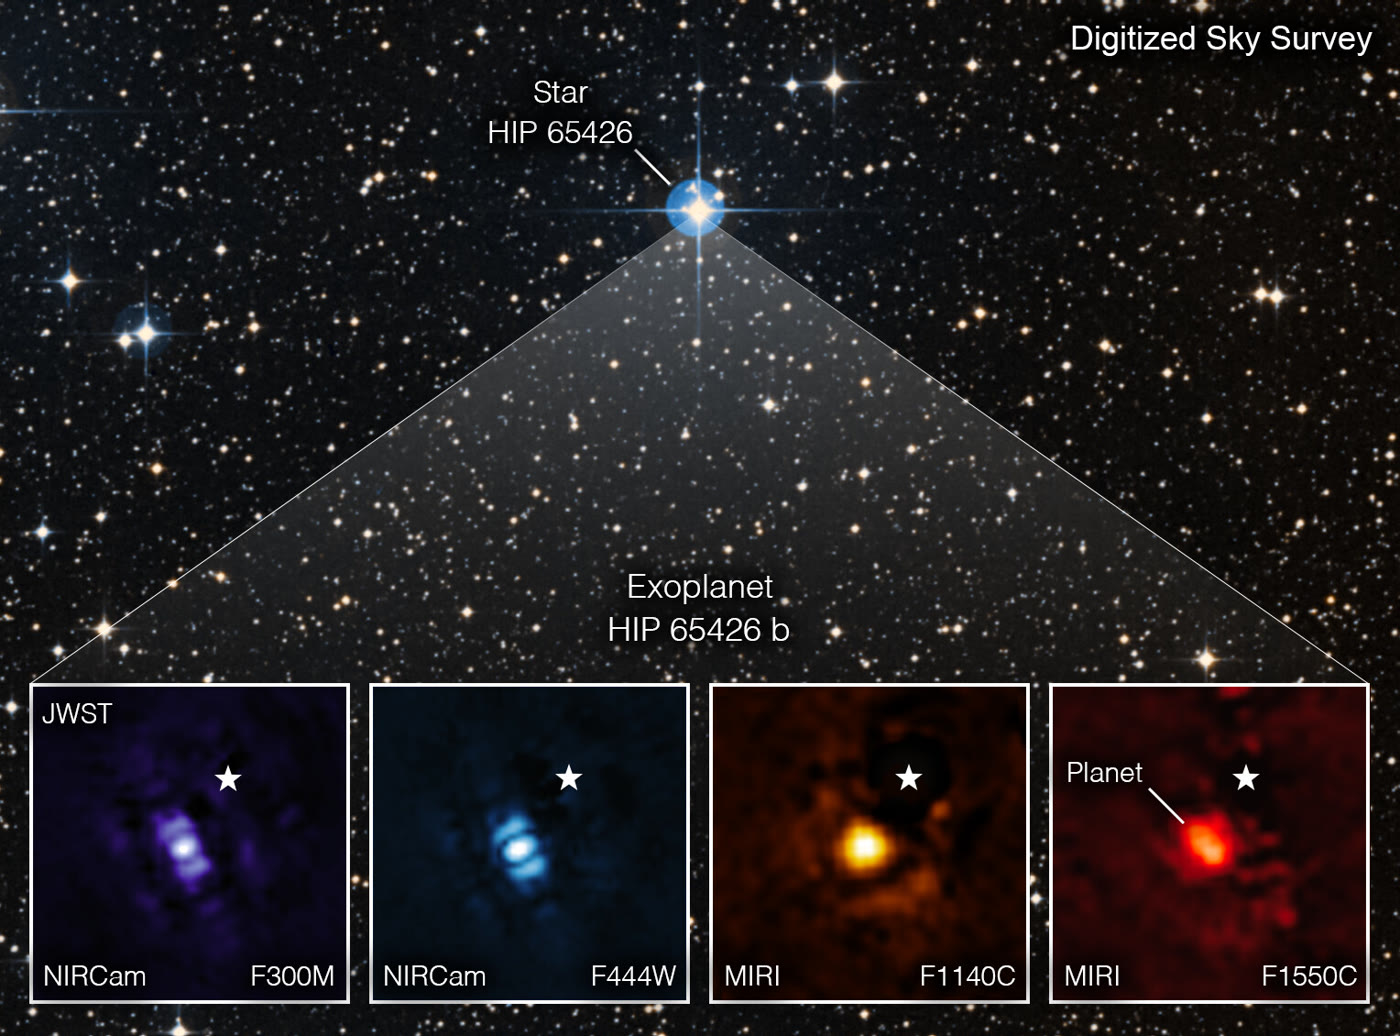
\includegraphics[width=0.86\linewidth]{images/book5/b3-hip65426b.jpg}
\par\smallskip{\small Eksoplanet pertama yang dicitrakan oleh James Webb Space
Telescope, HIP~65426~b, dalam empat filter inframerah (bawah; atas, medan
bintang dalam survei langit berbasis darat); cahaya
bintang, pada posisi simbol bintang, dihalangi oleh
\omterm{def:b3:exoplanets:imaging}{koronagraf}. Planet ini adalah raksasa gas muda, sekitar 6 hingga 8
massa Jupiter, berumur sekitar 15 hingga 20 juta tahun, kira-kira seratus kali
lebih jauh dari bintangnya daripada Bumi dari Matahari. Citra NASA/ESA/CSA,
A~Carter (UCSC), tim ERS~1386, dan A.~Pagan (STScI), CC
BY~4.0.}\label{fig:b3:exoplanets:hip65426}
\end{omfigure}
% ledger: photo:b3-hip65426b

Metode keempat menggunakan gravitasi sebagai lensa. Ketika sebuah bintang melintas hampir tepat
di depan bintang yang lebih jauh, gravitasinya membelokkan cahaya
bintang latar dan membuatnya lebih terang selama beberapa minggu; planet bintang pelensa
menambahkan kilatan singkat.

\begin{definition}[Pelensaan mikro gravitasi; jari-jari Einstein]\label{def:b3:exoplanets:microlensing}
Yang disebut \emph{pelensaan mikro gravitasi}\index{pelensaan mikro gravitasi} adalah
peningkatan kecerahan sementara bintang latar ketika bintang depan, lensanya,
melintas dekat garis pandang; citra yang dibentuknya terlalu dekat
berdekatan sehingga tidak dapat dipisahkan. Yang disebut \emph{jari-jari Einstein}\index{jari-jari Einstein}
adalah jari-jari sudut $\theta_\mathrm E$ cincin tempat lensa titik
bermassa $M$ pada jarak $D_L$ akan membelokkan sumber pada jarak $D_S$ tepat
di belakangnya:
\[
\theta_\mathrm E = \sqrt{\frac{4GM}{c^2}\,\frac{D_S - D_L}{D_L D_S}} .
\]
\end{definition}

\begin{proposition}[Pembesaran lensa titik]\label{prop:b3:exoplanets:magnification}
Sumber pada jarak sudut $u\,\theta_\mathrm E$ dari lensa titik
kecerahannya meningkat dengan faktor
\[
A(u) = \frac{u^2 + 2}{u\sqrt{u^2 + 4}} .
\]
\end{proposition}

\admitted

    Kedua hasil ini berasal dari pembelokan cahaya oleh massa dalam
    relativitas umum. Untuk lensa bermassa setengah massa Matahari yang berada di tengah jalan menuju sumber
    sejauh \qty{8}{kpc}, $\theta_\mathrm E = \qty{0.71}{mas}$, dan cincin
    Einstein pada jarak lensa memiliki jari-jari \qty{2.9}{au}. Pada
    $u = 1$ sumber menjadi 1.34 kali lebih terang, dan pada $u = 0.1$ sepuluh kali. Sebuah
    planet yang dekat cincin Einstein bintangnya menambahkan penyimpangan singkat pada
    kurva cahaya. Pelensaan mikro dengan demikian menemukan planet beberapa satuan astronomi
    dari bintangnya, planet dingin yang luput dari transit dan kecepatan radial,
    tetapi setiap kejadian hanya terjadi sekali dan tidak pernah berulang. Dalam sebuah kejadian pada 2003,
    yang dipublikasikan tahun berikutnya, penyimpangan selama sekitar tujuh hari
    hanya dijelaskan oleh pendamping bermassa $\num{0.0039}$ kali massa dari
    lensa: sebuah planet bermassa sekitar 1.5 massa Yupiter pada sekitar \qty{3}{au} dari
    bintangnya.
% ledger: const:G, const:c, sun:mass, iau:parsec, const:au, bond04:ogle235

\begin{omfigure}
\centering
\begin{tikzpicture}[scale=0.95]
\fill (0,0) circle (0.06) node[below=2pt, font=\scriptsize] {sumber};
\fill[omDef] (3.2,0) circle (0.09); \node[font=\scriptsize, omDef] at (3.2,-1.15) {lensa};
\draw[omDef] (3.2,0) ellipse (0.12 and 0.9);
\fill (6.4,0) circle (0.06) node[below=2pt, font=\scriptsize] {pengamat};
\draw[thick, orange!80!black] (0,0) -- (3.2,0.9) -- (6.4,0);
\draw[thick, orange!80!black] (0,0) -- (3.2,-0.9) -- (6.4,0);
\draw[densely dashed, black!50] (6.4,0) -- (0,1.8) node[left, font=\scriptsize] {citra};
\draw[densely dotted, black!50] (0,0) -- (6.4,0);
\draw[<->] (3.55,0) -- (3.55,0.9) node[midway, right, font=\scriptsize] {$R_\mathrm E$};
\draw[<->, black!60] (0,-1.5) -- (3.2,-1.5) node[midway, below, font=\scriptsize] {$D_S - D_L$};
\draw[<->, black!60] (3.2,-1.5) -- (6.4,-1.5) node[midway, below, font=\scriptsize] {$D_L$};
\end{tikzpicture}\hfill
\begin{tikzpicture}
\begin{axis}[width=0.48\linewidth, height=0.42\linewidth,
  xmin=-3, xmax=3, ymin=0.8, ymax=12, ymode=log,
  ytick={1,2,5,10}, yticklabels={1,2,5,10},
  xlabel={waktu ($t_\mathrm E$)}, ylabel={pembesaran $A$},
  tick label style={font=\scriptsize}, label style={font=\small},
  legend style={font=\scriptsize, at={(0.5,-0.30)}, anchor=north, legend columns=3, draw=none, cells={anchor=west}, /tikz/every even column/.append style={column sep=1em}}]
\addplot[thick, omDef] table[x=t_tE, y=A01] {figdata/out/bachelor-3-rv_transit-lens.dat};
\addlegendentry{$u_0 = 0.1$}
\addplot[thick, dashed, red!70!black] table[x=t_tE, y=A03] {figdata/out/bachelor-3-rv_transit-lens.dat};
\addlegendentry{$0.3$}
\addplot[thick, dotted, black] table[x=t_tE, y=A10] {figdata/out/bachelor-3-rv_transit-lens.dat};
\addlegendentry{$1$}
\end{axis}
\end{tikzpicture}
\par\smallskip{\small Kiri: geometri lensa gravitasi, tidak dalam
skala; sinar dari sumber melewati lensa kira-kira pada \omterm{def:b3:exoplanets:microlensing}{jari-jari Einstein}
$R_\mathrm E = \theta_\mathrm E D_L$ dan mencapai pengamat yang melihat
sumber yang tergeser ke citra. Kanan: pembesaran sumber titik oleh lensa
titik terhadap waktu, dalam satuan waktu $t_\mathrm E$ yang ditempuh lensa
untuk bergerak sejauh satu \omterm{def:b3:exoplanets:microlensing}{jari-jari Einstein}, untuk tiga jarak
pendekatan terdekat $u_0$ (dalam \omterm{def:b3:exoplanets:microlensing}{jari-jari Einstein}).}\label{fig:b3:exoplanets:microlensing}
\end{omfigure}

Setiap metode memiliki biasnya sendiri, dan katalog planet yang diketahui
mencerminkannya. \omterm{def:b3:exoplanets:rv}{Metode kecepatan radial} lebih menyukai planet bermassa besar yang dekat dengan
bintangnya; transit lebih menyukai planet besar yang dekat bintangnya, dan memerlukan
orbit yang sejajar garis pandang; pelensaan mikro menemukan planet pada beberapa satuan astronomi;
pencitraan menemukan raksasa muda pada puluhan atau ratusan satuan astronomi jauhnya.
Gambar di bawah menunjukkan hasilnya: setiap metode mengisi wilayahnya sendiri, dan
planet Tata Surya sebagian besar jatuh di celah-celah di antaranya.

\begin{dated}{2026}
Pada 23 Oktober 2026 NASA Exoplanet Archive mencatat 6451 planet
terkonfirmasi. Menurut metode penemuan: 4785 melalui transit, 1204 melalui kecepatan
radial, 292 melalui pelensaan mikro, 98 melalui pencitraan, 29 melalui \omterm{def:b3:exoplanets:ttv}{variasi
waktu transit}, dan sisanya dengan metode yang lebih langka, di antaranya yang paling awal dari semuanya,
ditemukan pada 1992 di sekitar pulsar melalui pengamatan waktu denyutnya. Penemuan pertama
dengan kecepatan radial berasal dari 1995, dengan transit dari 2002, dengan
pelensaan mikro dan pencitraan dari 2004.
\end{dated}
% ledger: data:b5-pscomp

\begin{omfigure}
\centering
\begin{tikzpicture}
\begin{axis}[width=0.86\linewidth, height=0.56\linewidth,
  xmode=log, ymode=log, xmin=0.004, xmax=2000, ymin=0.02, ymax=1e5,
  legend image post style={scale=2.2},
  xlabel={sumbu semimayor (au)}, ylabel={massa atau massa minimum ($M_\oplus$)},
  tick label style={font=\scriptsize}, label style={font=\small},
  legend style={font=\scriptsize, at={(0.5,-0.20)}, anchor=north, legend columns=4, draw=none, cells={anchor=west}, /tikz/every even column/.append style={column sep=1em}}]
\addplot[only marks, mark=*, mark size=0.6pt, omDef, opacity=0.6] table[x=a_au, y=mass] {figdata/out/bachelor-3-exoplanet_archive-ma-tr.dat};
\addlegendentry{transit}
\addplot[only marks, mark=*, mark size=0.6pt, red!70!black, opacity=0.6] table[x=a_au, y=mass] {figdata/out/bachelor-3-exoplanet_archive-ma-rv.dat};
\addlegendentry{kecepatan radial}
\addplot[only marks, mark=triangle*, mark size=1.2pt, green!45!black] table[x=a_au, y=mass] {figdata/out/bachelor-3-exoplanet_archive-ma-ml.dat};
\addlegendentry{pelensaan mikro}
\addplot[only marks, mark=diamond*, mark size=1.5pt, orange!85!black] table[x=a_au, y=mass] {figdata/out/bachelor-3-exoplanet_archive-ma-im.dat};
\addlegendentry{pencitraan}
\addplot[only marks, mark=square*, mark size=1.6pt, black, forget plot] table[x=a_au, y=mass] {figdata/out/bachelor-3-exoplanet_archive-solar.dat};
\node[font=\scriptsize, anchor=west, fill=white, inner sep=1pt] at (axis cs:1.15,1.0) {Bumi};
\node[font=\scriptsize, anchor=east, fill=white, inner sep=1pt] at (axis cs:0.63,0.82) {Venus};
\node[font=\scriptsize, anchor=east, fill=white, inner sep=1pt] at (axis cs:0.34,0.055) {Merkurius};
\node[font=\scriptsize, anchor=west, fill=white, inner sep=1pt] at (axis cs:1.75,0.107) {Mars};
\node[font=\scriptsize, anchor=west, fill=white, inner sep=1pt] at (axis cs:6.0,318) {Yupiter};
\node[font=\scriptsize, anchor=west, fill=white, inner sep=1pt] at (axis cs:11,95) {Saturnus};
\node[font=\scriptsize, anchor=north, fill=white, inner sep=1pt] at (axis cs:25,11) {Uranus, Neptunus};
\end{axis}
\end{tikzpicture}
\par\smallskip{\small Planet terkonfirmasi dengan massa terukur (atau \omterm{def:b3:exoplanets:rv}{massa
minimum}) dan sumbu semimayor, menurut metode penemuan (NASA Exoplanet
Archive, 23 Oktober 2026: 1691 melalui transit, 1151 melalui kecepatan radial, 286
melalui pelensaan mikro, 94 melalui pencitraan), beserta planet Tata Surya (persegi hitam
). Massa yang diprediksi dari \omterm{def:b3:exoplanets:mass-radius}{relasi massa--jari-jari} tidak disertakan. Penelitian ini
memanfaatkan NASA Exoplanet Archive, yang dioperasikan oleh
California Institute of Technology, berdasarkan kontrak dengan National
Aeronautics and Space Administration di bawah Exoplanet Exploration
Program.}\label{fig:b3:exoplanets:methods}
\end{omfigure}
% ledger: data:b5-pscomp, planet:Mercury.mass, planet:Venus.mass, planet:Earth.mass, planet:Mars.mass, planet:Jupiter.mass, planet:Saturn.mass, planet:Uranus.mass, planet:Neptune.mass, planet:Mercury.dist, planet:Venus.dist, planet:Earth.dist, planet:Mars.dist, planet:Jupiter.dist, planet:Saturn.dist, planet:Uranus.dist, planet:Neptune.dist

\section{Yang telah ditemukan}\label{sec:b3:exoplanets:found}

Kejutan pertama adalah \omterm{def:b3:exoplanets:classes}{Jupiter panas}, yakni planet raksasa dengan orbit
berperiode beberapa hari. 51~Pegasi~b tidak mungkin terbentuk sedekat itu dengan bintangnya; ia harus
terbentuk lebih jauh, mungkin pada beberapa satuan astronomi, di luar garis salju
cakramnya, lalu bermigrasi ke dalam melalui interaksinya dengan
cakram, sebagaimana diprediksi teori.
% ledger: nobel19:migration

\begin{definition}[Jupiter panas; super-Bumi; sub-Neptunus]\label{def:b3:exoplanets:classes}
Sebuah \emph{Jupiter panas}\index{Jupiter panas} adalah planet raksasa pada orbit dekat,
biasanya didefinisikan sebagai \omterm{def:b3:exoplanets:rv}{massa minimum} di atas 0.1 massa Jupiter dan periode
lebih pendek dari sepuluh hari. Sebuah \emph{super-Bumi}\index{super-Bumi} adalah planet
yang lebih besar dari Bumi tetapi lebih kecil dari \omterm{def:b3:exoplanets:radius-valley}{lembah jari-jari}, yakni hingga
sekitar 1.5 hingga 2 jari-jari Bumi, dan kemungkinan besar berupa batuan. Sebuah \emph{sub-Neptunus}\index{sub-Neptunus}
adalah planet di atas \omterm{def:b3:exoplanets:radius-valley}{lembah jari-jari} tetapi lebih kecil dari Neptunus, sekitar 2 hingga
4 jari-jari Bumi, yang jari-jarinya menuntut selubung gas ringan atau
zat volatil.
\end{definition}
% ledger: wright12:hj, fulton17:gap, planet:Neptune.diameter, planet:Earth.diameter

\begin{definition}[Laju kemunculan]\label{def:b3:exoplanets:occurrence}
Yang disebut \emph{laju kemunculan}\index{laju kemunculan} suatu kelas planet adalah
rata-rata jumlah planet semacam itu per bintang, atau pecahan bintang yang
memiliki satu, dalam rentang ukuran (atau massa) dan periode tertentu, setelah
hitungan suatu survei dikoreksi terhadap planet yang tidak dapat dideteksinya:
yakni planet yang orbitnya tidak sejajar untuk transit, dan planet yang terlalu kecil atau
terlalu jauh untuk diamati.
\end{definition}

\omterm{def:b3:exoplanets:classes}{Jupiter panas}, yang menonjol dalam katalog karena paling mudah
ditemukan, tergolong langka: survei \omterm{def:b3:exoplanets:rv}{metode kecepatan radial} terhadap bintang mirip Matahari terdekat menemukan
mereka di sekitar \qty[separate-uncertainty=true]{1.2 \pm 0.38}{\percent} bintang. Planet kecil tergolong
umum. Penelusuran kurva cahaya \num{42000} bintang yang diamati oleh
teleskop antariksa Kepler, satu studi menemukan 603 planet, sepuluh di antaranya berukuran Bumi (1 hingga 2
jari-jari Bumi) dan menerima satu hingga empat kali cahaya Matahari yang diterima Bumi;
setelah dikoreksi terhadap peluang transit dan terhadap planet yang luput dari
pencarian, \qty[separate-uncertainty=true]{11 \pm 4}{\percent} bintang mirip Matahari memiliki
planet semacam itu.
% ledger: wright12:hj, petigura13:eta

Ukuran planet kecil tidak tersebar merata. Di antara planet dekat yang
diukur dengan teliti, yang berjari-jari 1.5 hingga 2.0 jari-jari Bumi setidaknya dua kali
lebih jarang daripada yang sedikit lebih kecil atau sedikit lebih besar.

\begin{definition}[Lembah jari-jari]\label{def:b3:exoplanets:radius-valley}
Yang disebut \emph{lembah jari-jari}\index{lembah jari-jari} adalah kekurangan planet
berjari-jari antara sekitar 1.5 dan 2.0 jari-jari Bumi di antara planet dengan
periode kurang dari sekitar seratus hari; ia memisahkan \omterm{def:b3:exoplanets:classes}{super-Bumi}
dari \omterm{def:b3:exoplanets:classes}{sub-Neptunus}.
\end{definition}
% ledger: fulton17:gap

Lembah ini ditafsirkan sebagai jejak lolosnya. Inti berbatuan yang lahir dengan
selubung hidrogen dan helium yang hanya beberapa persen massanya memiliki dua kali
jari-jari inti telanjangnya. Di dekat bintang muda yang aktif, selubung
semacam itu dipanaskan dan lepas melalui \omterm{def:b3:planetary-atmospheres:hydrodynamic}{lolos hidrodinamik}: oleh
radiasi berenergi tinggi bintang selama seratus juta tahun pertama
(fotoevaporasi), atau oleh panas dari inti yang sedang mendingin (kehilangan
massa bertenaga inti). Model-model menggiring planet ke inti telanjang sekitar 1.3 jari-jari Bumi
dan ke planet berukuran dua kali lipatnya; sedikit yang tersisa di antara keduanya. Kedua
mekanisme itu bergantung berbeda pada bintangnya, dan planet di sekitar bintang
berbeda jenis mungkin dapat membedakannya.
% ledger: owen17:valley, ginzburg18:core-powered

\begin{omfigure}
\centering
\begin{tikzpicture}
\begin{axis}[name=pr, width=0.50\linewidth, height=0.50\linewidth,
  xmode=log, ymode=log, xmin=1, xmax=100, ymin=0.8, ymax=4,
  ytick={1,1.5,2,3,4}, yticklabels={1,1.5,2,3,4},
  xlabel={periode (hari)}, ylabel={jari-jari ($R_\oplus$)},
  tick label style={font=\scriptsize}, label style={font=\small},
  title={(a)}, title style={font=\small}]
\fill[black!10] (axis cs:1,1.5) rectangle (axis cs:100,2.0);
\addplot[only marks, mark=*, mark size=0.5pt, omDef, opacity=0.7] table[x=period, y=radius] {figdata/out/bachelor-3-exoplanet_archive-pr.dat};
\end{axis}
\begin{axis}[at={(pr.east)}, anchor=west, xshift=0.09\linewidth,
  width=0.42\linewidth, height=0.50\linewidth,
  xmode=log, xmin=0.8, xmax=4, ymin=0, ymax=185,
  xtick={1,1.5,2,3,4}, xticklabels={1,1.5,2,3,4},
  xlabel={jari-jari ($R_\oplus$)}, ylabel={jumlah planet},
  tick label style={font=\scriptsize}, label style={font=\small},
  title={(b)}, title style={font=\small}]
\fill[black!10] (axis cs:1.5,0) rectangle (axis cs:2.0,185);
\addplot[const plot mark left, thick, omDef, fill=omDef!25] table[x=r, y=n] {figdata/out/bachelor-3-exoplanet_archive-histstep.dat} \closedcycle;
\end{axis}
\end{tikzpicture}
\par\smallskip{\small (a)~Planet transit dengan jari-jari yang diketahui lebih baik
daripada \qty{10}{\percent}, di sekitar bintang yang lebih kecil dari dua jari-jari Matahari,
dengan periode 1 hingga 100 hari (2370 planet, NASA Exoplanet Archive, 23
Oktober 2026); yang diarsir, \omterm{def:b3:exoplanets:radius-valley}{lembah jari-jari} 1.5 hingga 2.0 jari-jari Bumi.
(b)~Planet yang sama dihitung dalam 20 bin dengan lebar sama dalam $\log R$.
Hitungan ini tidak dikoreksi terhadap planet yang luput dari survei, yang
jumlahnya lebih banyak di antara yang kecil; lembah tetap terlihat.}\label{fig:b3:exoplanets:valley}
\end{omfigure}
% ledger: data:b5-pscomp, fulton17:gap

\begin{definition}[Relasi massa--jari-jari]\label{def:b3:exoplanets:mass-radius}
Yang disebut \emph{relasi massa--jari-jari}\index{relasi massa--jari-jari} suatu
komposisi adalah jari-jari planet dengan komposisi tersebut sebagai fungsi
massanya, dihitung dari persamaan keadaan bahan-bahannya dalam
kesetimbangan hidrostatik; planet yang terukur dibandingkan dengan
relasi komposisi kandidat.
\end{definition}

Planet batuan dimampatkan oleh beratnya sendiri, dan jari-jarinya tumbuh
lebih lambat daripada $M^{1/3}$. Kecocokan terhadap model planet dua lapis yang dibangun di atas
model seismik Bumi menghasilkan $R/R_\oplus = (1.07 - 0.21\,C)
(M/M_\oplus)^{1/3.7}$, untuk 1 hingga 8 massa Bumi dan fraksi massa inti
$C$ dari 0 hingga 0.4; dicocokkan dengan Bumi, Venus, dan beberapa eksoplanet kecil,
ia menghasilkan $C = 0.26 \pm 0.07$. Sebuah
planet besi lebih kecil pada massa yang sama; planet separuh air, lebih besar;
selubung hidrogen yang hanya dua persen massanya membuat planet
lima massa Bumi dan berjari-jari \num{2.6} jari-jari Bumi, sebesar
\omterm{def:b3:exoplanets:classes}{sub-Neptunus}. Degenerasi ini nyata: satu jari-jari dan satu massa memberikan satu
massa jenis, dan beberapa campuran besi, batuan, air, dan gas dapat memilikinya.
Planet batuan Kepler-10~b, dengan massa 3.24 massa Bumi dan jari-jari 1.47 jari-jari Bumi,
memiliki massa jenis rata-rata \qty{5.6}{g.cm^{-3}}; raksasa gas WASP-39~b,
dengan massa 89 massa Bumi dan jari-jari 14.3 jari-jari Bumi, memiliki \qty{0.17}{g.cm^{-3}}.
% ledger: zeng16:rocky, data:b5-zeng, data:b5-pscomp

\begin{omfigure}
\centering
\begin{tikzpicture}
\begin{axis}[width=0.86\linewidth, height=0.58\linewidth,
  xmode=log, ymode=log, xmin=0.3, xmax=5000, ymin=0.5, ymax=25,
  ytick={0.5,1,2,4,10,20}, yticklabels={0.5,1,2,4,10,20},
  xlabel={massa ($M_\oplus$)}, ylabel={jari-jari ($R_\oplus$)},
  tick label style={font=\scriptsize}, label style={font=\small},
  legend style={font=\scriptsize, at={(0.5,-0.20)}, anchor=north, legend columns=3, draw=none, cells={anchor=west}, /tikz/every even column/.append style={column sep=1em}}]
\addplot[only marks, mark=*, mark size=0.6pt, black!35, forget plot] table[x=mass, y=radius] {figdata/out/bachelor-3-exoplanet_archive-mr.dat};
\addplot[thick, black] table[x=mass, y=radius] {figdata/out/bachelor-3-exoplanet_archive-zeng-iron.dat};
\addlegendentry{besi murni}
\addplot[thick, brown!70!black] table[x=mass, y=radius] {figdata/out/bachelor-3-exoplanet_archive-zeng-earthlike.dat};
\addlegendentry{batuan mirip Bumi}
\addplot[thick, omDef] table[x=mass, y=radius] {figdata/out/bachelor-3-exoplanet_archive-zeng-water50.dat};
\addlegendentry{50\,\% air}
\addplot[thick, dashed, orange!85!black] table[x=mass, y=radius] {figdata/out/bachelor-3-exoplanet_archive-zeng-h2-2pc.dat};
\addlegendentry{batuan + 2\,\% hidrogen}
\addplot[only marks, mark=square*, mark size=1.8pt, red!70!black] table[x=mass, y=radius] {figdata/out/bachelor-3-exoplanet_archive-solar.dat};
\addlegendentry{Tata Surya}
\node[font=\scriptsize, anchor=north west] at (axis cs:1.05,0.97) {Bumi};
\node[font=\scriptsize, anchor=south east] at (axis cs:0.80,0.97) {Venus};
\node[font=\scriptsize, anchor=south east, fill=white, inner sep=1pt] at (axis cs:13.5,4.3) {Uranus, Neptunus};
\node[font=\scriptsize, anchor=east, fill=white, inner sep=1pt] at (axis cs:80,9.45) {Saturnus};
\node[font=\scriptsize, anchor=north, fill=white, inner sep=1pt] at (axis cs:318,10.3) {Jupiter};
\end{axis}
\end{tikzpicture}
\par\smallskip{\small Massa dan jari-jari 1078 planet transit yang
massanya terukur dengan galat kurang dari \qty{25}{\percent} dan jari-jarinya dengan galat
kurang dari \qty{10}{\percent} (abu-abu; NASA Exoplanet Archive, 23 Oktober 2026),
dengan kurva model dari L.~Zeng dkk. (2016, 2019): besi murni;
batuan mirip Bumi, sepertiga besi dan dua pertiga silikat; separuh air di atas
inti seperti itu, pada \qty{500}{K}; inti mirip Bumi dengan selubung hidrogen sebesar
\qty{2}{\percent} massanya, pada \qty{500}{K}. Kotak merah: planet-planet Tata
Surya (Merkurius dan Mars berada di luar skala, di sebelah
kiri).}\label{fig:b3:exoplanets:mass-radius}
\end{omfigure}
% ledger: data:b5-pscomp, data:b5-zeng, planet:Earth.mass, planet:Earth.diameter, planet:Venus.mass, planet:Venus.diameter, planet:Jupiter.mass, planet:Jupiter.diameter, planet:Saturn.mass, planet:Saturn.diameter, planet:Uranus.mass, planet:Uranus.diameter, planet:Neptune.mass, planet:Neptune.diameter

\section{Atmosfer}\label{sec:b3:exoplanets:atmospheres}

Planet transit dapat ditimbang dan diukur; planet itu juga dapat diendus.
Selama transit, cincin tipis atmosfer planet berdiri menghadap
bintang, dan cahaya bintang menyaring melalui cincin itu. Pada panjang gelombang tempat gas
atmosfer menyerap, cincin itu buram hingga ke ketinggian yang lebih besar, dan planet
tampak lebih besar.

\begin{definition}[Spektroskopi transmisi; gerhana sekunder]\label{def:b3:exoplanets:transmission}
Yang disebut \emph{spektroskopi transmisi}\index{spektroskopi transmisi} mengukur
\omterm{def:b3:exoplanets:transit}{kedalaman transit} sebagai fungsi panjang gelombang, untuk mendeteksi gas
atmosfer yang dilintasi cahaya bintang di tepi planet. Sebuah
\emph{gerhana sekunder}\index{gerhana sekunder} adalah lintasan
planet di belakang bintangnya, setengah orbit setelah transit pada orbit
melingkar; penurunan fluks sistem kemudian mengukur cahaya
sisi siang planet.
\end{definition}

\begin{proposition}[Sinyal transmisi]\label{prop:b3:exoplanets:transmission}
Atmosfer dengan tinggi skala $H \ll R_p$ yang dibuat buram sepanjang $n$ tinggi
skala tambahan pada panjang gelombang pita serapan dibanding pada
panjang gelombang tetangga, memperdalam transit di sana sebesar
\[
\Delta\delta \approx n\,\frac{2HR_p}{R_\star^2} .
\]
\end{proposition}

\begin{proof}
Jari-jari tampak planet membesar dari $R_p$ menjadi $R_p + nH$, sehingga
kedalaman $(R_p + nH)^2/R_\star^2$ bertambah sebesar $(2nHR_p + n^2H^2)/R_\star^2$,
yaitu $2nHR_p/R_\star^2$ bila $nH \ll R_p$.
\end{proof}

Tinggi skala $H = kT/\bar m g$ besar bagi planet panas dengan gravitasi rendah
dengan udara ringan berbasis hidrogen, dan kecil bagi planet dingin dan padat dengan
udara berat. Untuk Bumi yang dilihat di depan Matahari, dengan $H = \qty{8}{km}$,
setiap tinggi skala menambah 0.2 bagian per juta; untuk raksasa gas panas yang menggembung,
beberapa ratus.
% ledger: planet:Earth.diameter, sun:R

\begin{proposition}[Kedalaman gerhana sekunder]\label{prop:b3:exoplanets:eclipse}
Jika sisi siang planet memancar sebagai benda hitam pada suhu
$T_d$ dan bintang sebagai benda hitam pada $T_\star$, \omterm{def:b3:exoplanets:transmission}{gerhana sekunder} pada
panjang gelombang $\lambda$ memiliki kedalaman
\[
\delta_\mathrm{ecl} \approx \left(\frac{R_p}{R_\star}\right)^2
  \frac{B_\lambda(T_d)}{B_\lambda(T_\star)},
\]
dengan $B_\lambda$ hukum Planck, dan cahaya pantul planet diabaikan.
\end{proposition}

\begin{proof}
Tepat sebelum gerhana, pengamat menerima cahaya bintang, sebanding
dengan $\pi R_\star^2 B_\lambda(T_\star)$, ditambah cahaya sisi siang,
sebanding dengan $\pi R_p^2 B_\lambda(T_d)$; selama gerhana hanya
cahaya bintang. Penurunan pecahannya adalah rasio suku planet terhadap
suku bintang, sebab planet itu kecil.
\end{proof}

Gerhana paling dalam di inframerah, tempat planet yang dingin
paling terang relatif terhadap bintangnya: gerhana itu memberikan suhu sisi siang,
sisi siang yang panas di samping sisi malam yang dingin menunjukkan atmosfer
tipis atau tidak ada yang tidak menyalurkan panas.

\begin{dated}{2023}
Pada 2022 spektrum transmisi raksasa gas WASP-39~b, yang diukur
antara 3.0 dan \qty{5.5}{\micro m} oleh James Webb Space Telescope,
menunjukkan pita serapan karbon dioksida yang menonjol pada
\qty{4.3}{\micro m}, pada 26 simpangan baku, padahal fotometri sebelumnya
hanya mengisyaratkan gas itu: ini identifikasi jelas pertama di
atmosfer eksoplanet. Pada 2023 lima \omterm{def:b3:exoplanets:transmission}{gerhana sekunder} dari
TRAPPIST-1~b yang sebesar Bumi, menerima empat kali cahaya yang diterima Bumi
dari bintang kecil dan dingin, diukur pada \qty{15}{\micro m}. Data itu
sesuai dengan panas yang dipancarkan ulang dari sisi siang saja, tanpa karbon
dioksida yang terdeteksi: planet itu punya sedikit atau tidak ada atmosfer untuk
membawa panas ke sisi malamnya.
\end{dated}
% ledger: jwst23:wasp39-co2, greene23:trappist1b

Planet batuan di zona layak huni bintang kecil berada
dalam jangkauan metode-metode ini, meskipun di batas kemampuannya.
Apakah planet-planet itu mempertahankan udaranya terhadap proses lolos
pada bab sebelumnya kini menjadi pertanyaan observasional.

\section{Latihan}

\begin{exercise}[$\star$]\label{exo:b3:exoplanets:1}
(a)~Hitung amplitudo semi kecepatan radial Matahari yang disebabkan
oleh Jupiter (massa \qty{1898e24}{kg}, periode \num{4331}~hari, eksentrisitas
0.049) dan oleh Bumi (massa \qty{5.97e24}{kg}, periode \num{365.2}~hari,
eksentrisitas 0.017). Massa Matahari adalah \qty{1.9884e30}{kg}.
(b)~Ubah ketelitian \qty{3.5}{km/h} dan \qty{0.35}{km/h} menjadi
meter per detik, lalu bandingkan.
\end{exercise}

\begin{exercise}[$\star$]\label{exo:b3:exoplanets:2}
(a)~Hitung \omterm{def:b3:exoplanets:transit}{kedalaman transit} Jupiter (jari-jari \qty{71492}{km}) dan
Bumi (jari-jari \qty{6378}{km}) melintasi Matahari (jari-jari
\qty{695700}{km}). (b)~Hitung peluang pengamat yang ditempatkan secara acak
melihat masing-masing transit, dengan jari-jari orbit \num{778.5}
dan \qty{149.6}{\mega km}.
\end{exercise}

\begin{exercise}[$\star$]\label{exo:b3:exoplanets:3}
51~Pegasi~b memberi bintangnya amplitudo semi kecepatan radial
\qty{59}{m.s^{-1}}, dengan periode \qty{4.23}{d}. Anggap massa bintang sama
dengan massa Matahari, hitung \omterm{def:b3:exoplanets:rv}{massa minimum} planet itu, dalam massa Jupiter
dan massa Bumi, serta jari-jari orbitnya.
\end{exercise}

\begin{exercise}[$\star$]\label{exo:b3:exoplanets:4}
Sebuah bintang bermassa setengah massa Matahari pada \qty{4}{kpc} melensakan
sebuah bintang pada \qty{8}{kpc} ($\qty{1}{pc} = \qty{3.0857e16}{m}$). (a)~Hitung \omterm{def:b3:exoplanets:microlensing}{jari-jari Einstein-nya} dalam milidetik busur
dan jari-jari cincin Einstein, dalam satuan astronomi, pada jarak lensa. (b)~Hitung
magnifikasi pada $u = 1$, $0.5$ dan $0.1$. (c)~Berapa lama lensa itu
melintasi satu \omterm{def:b3:exoplanets:microlensing}{jari-jari Einstein} jika ia bergerak melintasi
garis pandang dengan kecepatan
\qty{200}{km.s^{-1}}?
\end{exercise}

\begin{exercise}[$\star\star$]\label{exo:b3:exoplanets:5}
Sebuah planet dengan rasio jari-jari $p = 0.12$ mengorbit bintang bermassa satu
massa Matahari dan berjari-jari satu jari-jari Matahari dalam \qty{3.0}{d}. (a)~Hitung $a/R_\star$. (b)~Hitung
$T_{14}$ dan $T_{23}$ untuk $b = 0$ dan untuk $b = 0.7$, serta inklinasi
pada kasus kedua. (c)~Bagaimana bentuk kurva cahaya membedakan transit pusat
dari transit yang menyerempet?
\end{exercise}

\begin{exercise}[$\star\star$]\label{exo:b3:exoplanets:6}
Dari massa dan jari-jari Exoplanet Archive, hitung massa jenis rata-rata
TRAPPIST-1~b (1.374 massa Bumi, 1.116 jari-jari Bumi),
Kepler-10~b (3.24, 1.47), WASP-39~b (89.31, 14.34) dan HD~209458~b (232.0,
15.58), dengan $M_\oplus = \qty{5.97e24}{kg}$ dan $R_\oplus =
\qty{6378}{km}$. Mana yang berbatuan, mana yang gas?
\end{exercise}

\begin{exercise}[$\star\star$]\label{exo:b3:exoplanets:7}
Kecepatan radial sebuah bintang dengan satu planet pada orbit eksentrik
berkisar dari $+\qty{50.4}{m.s^{-1}}$ hingga $-\qty{9.6}{m.s^{-1}}$, dan kecepatan
pusat massa sistem adalah \qty{12.4}{m.s^{-1}}. Dengan memakai bentuk eksentrik
teorema itu, hitung $K$ dan $e\cos\omega$. Mengapa rata-rata kedua ekstrem
dapat berbeda dari $\gamma$?
\end{exercise}

\begin{exercise}[$\star\star$]\label{exo:b3:exoplanets:8}
WASP-39~b memiliki massa 89.31 massa Bumi dan jari-jari 14.34 jari-jari Bumi;
bintangnya berjari-jari 0.939 jari-jari Matahari. Ambil suhu \qty{1100}{K} dan
massa molekul rata-rata \qty{2.3}{u} untuk atmosfernya. (a)~Hitung gravitasinya,
tinggi skalanya, dan \omterm{def:b3:exoplanets:transit}{kedalaman transitnya}. (b)~Hitung sinyal transmisi untuk
satu tinggi skala, dan untuk pita serapan yang tingginya dua tinggi skala,
dalam bagian per juta.
\end{exercise}

\begin{exercise}[$\star\star$]\label{exo:b3:exoplanets:9}
TRAPPIST-1~b memiliki jari-jari 1.116 jari-jari Bumi; bintangnya berjari-jari 0.1192
jari-jari Matahari dan bersuhu \qty{2566}{K}. Hitung kedalaman \omterm{def:b3:exoplanets:transmission}{gerhana sekunder} pada
\qty{15}{\micro m} untuk sisi siang bersuhu \qty{400}{K} dan \qty{500}{K}
($hc/k = \qty{0.014388}{m.K}$). Mengapa pengukuran kedalaman itu berfungsi
sebagai termometer?
\end{exercise}

\begin{exercise}[$\star\star\star$]\label{exo:b3:exoplanets:10}
Sebuah katai merah rekaan memiliki massa 0.2 massa Matahari, jari-jari 0.2 jari-jari Matahari,
dan luminositas \num{0.005} luminositas Matahari. (a)~Pada jarak berapa sebuah planet
menerima fluks bintang yang sama dengan Bumi, dan berapa periodenya?
(b)~Hitung amplitudo semi yang disebabkan oleh planet bermassa satu massa Bumi di sana,
lalu bandingkan dengan pengaruh Bumi terhadap Matahari. (c)~Hitung \omterm{def:b3:exoplanets:transit}{kedalaman transit}
planet sebesar Bumi. Mengapa bintang semacam ini menjadi target yang diutamakan
dalam pencarian planet batuan di zona layak huni?
\end{exercise}

\begin{exercise}[$\star\star\star$]\label{exo:b3:exoplanets:11}
Untuk hukum \omterm{def:b3:exoplanets:limb}{penggelapan tepi} kuadratik, tunjukkan bahwa intensitas rata-rata
cakram adalah $I(1)(1 - u_1/3 - u_2/6)$. Turunkan kedalaman, dalam satuan
$p^2$, dari planet kecil pada $r = 0$, $0.5$ dan $0.9$ untuk $u_1 = 0.40$,
$u_2 = 0.25$. Kesalahan apa yang dibuat model cakram seragam pada jari-jari
planet yang diamati pada tengah transit dengan $b = 0$?
\end{exercise}

\begin{exercise}[$\star\star\star$]\label{exo:b3:exoplanets:12}
Sebuah survei mengamati \num{42000} bintang mirip Matahari dan mencarinya untuk
planet sebesar Bumi yang menerima satu sampai empat kali sinar Matahari yang diterima Bumi,
yaitu pada orbit 0.5 sampai \qty{1}{au}. (a)~Hitung peluang transit
pada 0.5, 0.7 dan \qty{1}{au}. (b)~Jika \qty{11}{\percent} bintang menjadi tuan rumah
bagi satu planet seperti itu, pada sekitar \qty{0.7}{au}, berapa yang transit?
(c)~Survei itu menemukan sepuluh. Apa yang diukur oleh selisihnya, dan mengapa
\omterm{def:b3:exoplanets:occurrence}{laju kemunculan} harus dikoreksi karenanya?
\end{exercise}

\section{Soal: Planet di sekitar Lampu Selene}

\begin{problem}[{Soal akhir pekan --- menimbang, mengukur, dan mengendus
sebuah planet rekaan}]
\label{pb:b3:exoplanets:1}
Lampu Selene adalah katai~K rekaan bermassa 0.80 massa Matahari, jari-jari
0.76 jari-jari Matahari, dan suhu efektif \qty{5000}{K}. Sebuah survei
kecepatan radial menemukan bahwa kecepatan itu bervariasi secara sinusoidal
dengan periode \qty{12.0}{d} dan semi-amplitudo \qty{2.59}{m.s^{-1}}. Sebuah
teleskop antariksa kemudian mengamati transit dengan periode yang sama,
kedalaman \num{838} bagian per juta dan durasi total $T_{14} = \qty{3.23}{h}$.
Gunakan $M_\odot = \qty{1.9884e30}{kg}$, $R_\odot = \qty{695700}{km}$,
$L_\odot = \qty{3.828e26}{W}$, $M_\oplus = \qty{5.97e24}{kg}$,
$R_\oplus = \qty{6378}{km}$.

\medskip\noindent\textbf{Bagian I --- Kecepatan radial.}
\begin{enumerate}
\item Hitung jari-jari orbit, dalam meter dan dalam
  satuan astronomi, dengan mengabaikan massa planet terhadap massa bintang.
\item Hitung kelajuan orbit planet.
\item Hitung \omterm{def:b3:exoplanets:rv}{massa minimum} planet, dalam massa Bumi.
\item Hitung jari-jari orbit bintang itu sendiri mengelilingi pusat
  massa, dan periksa bahwa hasilnya memberikan semi-amplitudo yang teramati.
\item Berapa kali lipat sinyal melampaui presisi
  \qty{1}{m.s^{-1}} dan \qty{0.1}{m.s^{-1}}?
\item Jika orbitnya memiliki $e = 0.2$ dengan $K$ yang sama, berapa besar
  \omterm{def:b3:exoplanets:rv}{massa minimum} akan berubah?
\end{enumerate}

\medskip\noindent\textbf{Bagian II --- Transit.}
\begin{enumerate}[resume]
\item Hitung rasio jari-jari $p = R_p/R_\star$.
\item Hitung jari-jari planet, dalam kilometer dan dalam jari-jari Bumi.
\item Hitung $a/R_\star$.
\item Hitung durasi transit pusat ($b = 0$).
\item Dari $T_{14}$ yang teramati, hitung \omterm{def:b3:exoplanets:transit}{parameter tumbukan}.
\item Hitung inklinasi orbit.
\item Berapa peluang planet ini mengalami transit, jika dilihat dari arah
  acak?
\end{enumerate}

\medskip\noindent\textbf{Bagian III --- Apa penyusunnya?}
\begin{enumerate}[resume]
\item Hitung massa sejati planet.
\item Hitung massa jenis rata-rata planet.
\item Pada kurva model batuan mirip Bumi, planet bermassa ini akan
  memiliki jari-jari 1.74 jari-jari Bumi. Bandingkan, dan katakan apa yang harus
  dikandung planet itu selain batuan.
\item Di mana letak planet terhadap \omterm{def:b3:exoplanets:radius-valley}{lembah jari-jari}? Apakah itu
  \omterm{def:b3:exoplanets:classes}{super-Bumi} atau \omterm{def:b3:exoplanets:classes}{sub-Neptunus}?
\item Hitung percepatan gravitasi permukaannya.
\end{enumerate}

\medskip\noindent\textbf{Bagian IV --- Atmosfernya.}
\begin{enumerate}[resume]
\item Hitung luminositas bintang, dalam watt dan dalam
  luminositas Matahari.
\item Hitung fluks bintang yang diterima planet, relatif terhadap fluks
  yang diterima Bumi. Apakah planet ini berada di zona layak huni?
\item Dengan albedo Bond 0.3, hitung suhu kesetimbangannya.
\item Hitung tinggi skala atmosfer hidrogen dan helium
  (massa molekul rata-rata \qty{2.3}{u}) pada suhu tersebut.
\item Hitung sinyal transmisi untuk satu tinggi skala, dan untuk pita
  air setinggi dua tinggi skala, dalam bagian per juta.
\item Hitung hal yang sama untuk atmosfer uap air (\qty{18}{u}). Manakah dari
  keduanya yang dapat dibedakan teleskop antariksa dengan presisi sekitar sepuluh bagian per
  juta dari spektrum datar?
\item Berikan massa jenis rata-rata planet, dalam gram per sentimeter kubik, hingga
  dua angka penting.
\end{enumerate}
\end{problem}
% ledger: sun:mass, sun:R, sun:L, planet:Earth.mass, planet:Earth.diameter, const:G, const:kB, const:sigma, nist:u, data:b5-zeng, fulton17:gap, eso:espresso
